\section{Auswertung}
\label{sec:Auswertung}

\subsection{Fehlerrechnung}
\label{sec:Fehlerrechnung}
Für die Fehlerrechnung werden folgende Formeln aus der Vorlesung verwendet.
für den Mittelwert gilt
\begin{equation}
    \overline{x}=\frac{1}{N}\sum_{i=1}^N x_i ß\; \;\text{mit der Anzahl N und den Messwerten x} 
    \label{eqn:Mittelwert}
\end{equation}
Der Fehler für den Mittelwert lässt sich gemäß
\begin{equation}
    \increment \overline{x}=\frac{1}{\sqrt{N}}\sqrt{\frac{1}{N-1}\sum_{i=1}^N(x_i-\overline{x})^2}
    \label{eqn:FehlerMittelwert}
\end{equation}
berechnen.
Wenn im weiteren Verlauf der Berechnung mit der fehlerhaften Größe gerechnet wird, kann der Fehler der folgenden Größe
mittels Gaußscher Fehlerfortpflanzung berechnet werden. Die Formel hierfür ist
\begin{equation}
    \increment f= \sqrt{\sum_{i=1}^N\left(\frac{\partial f}{\partial x_i}\right)^2\cdot(\increment x_i)^2}.
    \label{eqn:GaussMittelwert}
\end{equation}

\begin{figure}
    \centering
    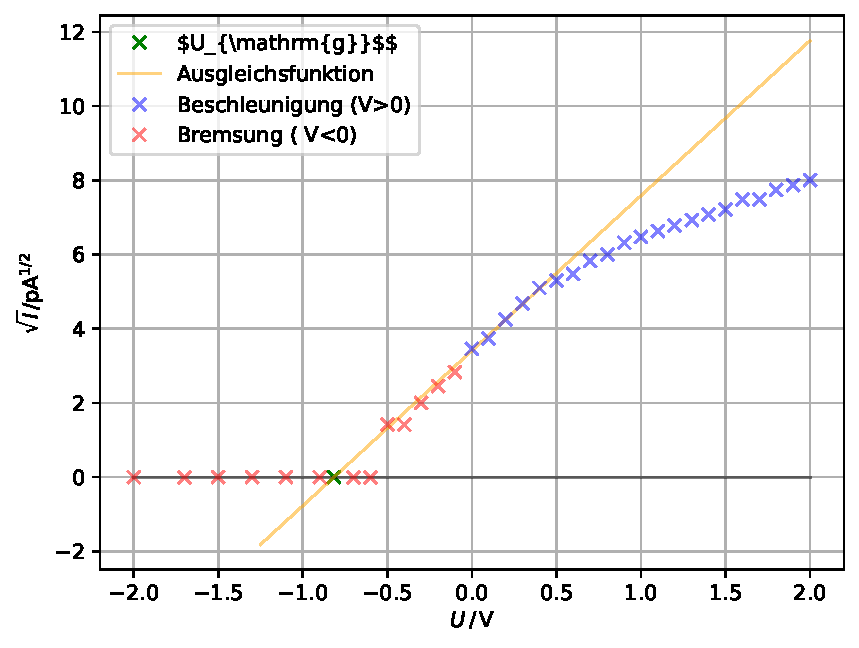
\includegraphics[height = 8cm]{build/plotrot.pdf}
    \caption{Regression zur Bestimmung der Grenzspannung $U_{\symup{g}}$ der roten Spektrallinie.}
    \label{fig:rot}
\end{figure}

\begin{figure}
    \centering
    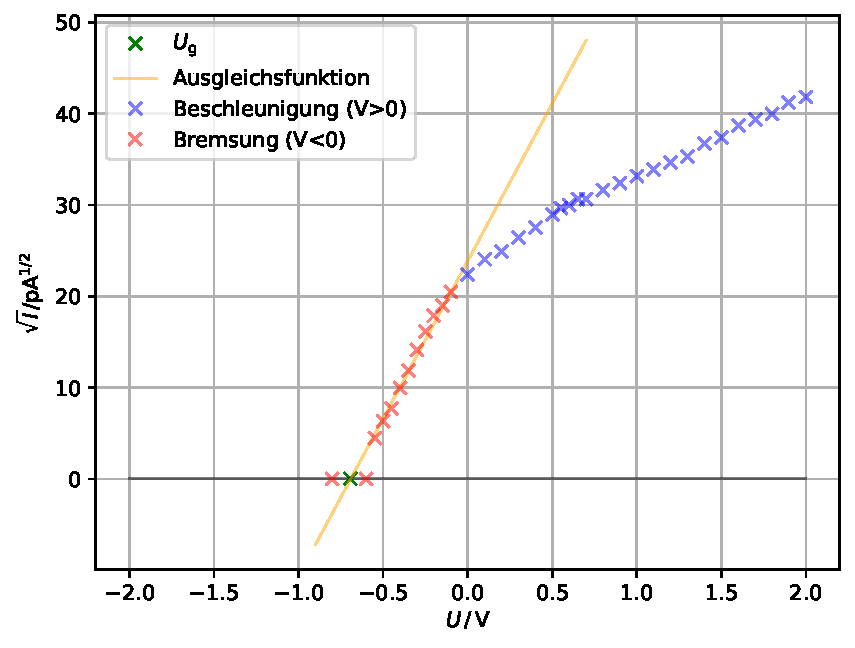
\includegraphics[height = 8cm]{build/plotgruen.pdf}
    \caption{Regression zur Bestimmung der Grenzspannung $U_{\symup{g}}$ der grünen Spektrallinie.}
    \label{fig:gruen}
\end{figure}

\begin{figure}
    \centering
    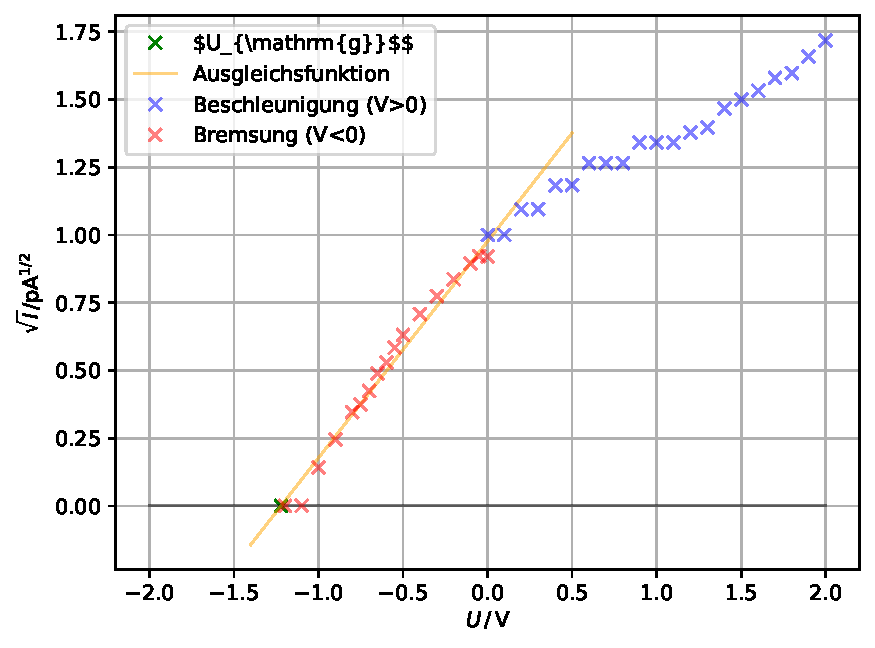
\includegraphics[height = 8cm]{build/plotlila.pdf}
    \caption{Regression zur Bestimmung der Grenzspannung $U_{\symup{g}}$ der violetten Spektrallinie.}
    \label{fig:lila}
\end{figure}

\begin{figure}
    \centering
    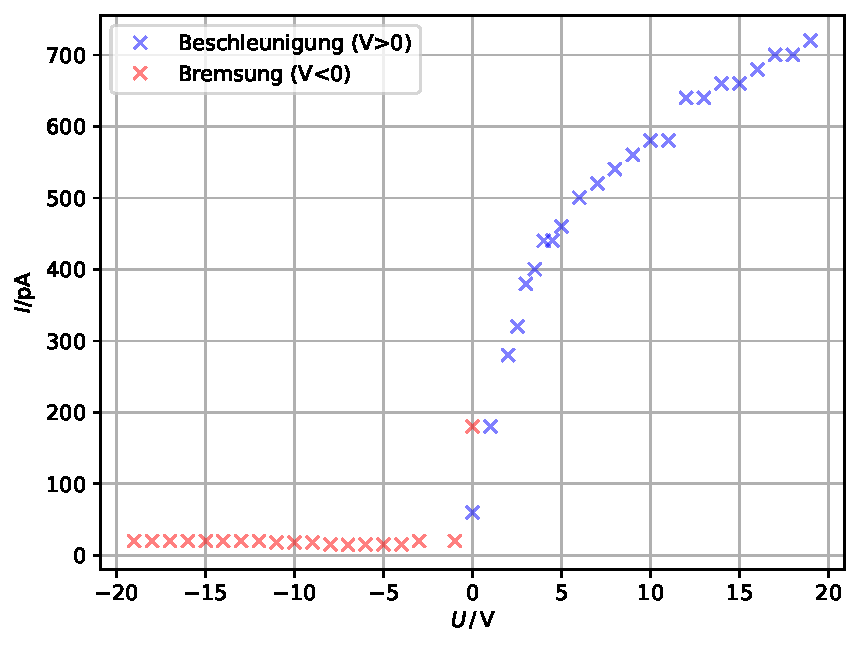
\includegraphics[height = 8cm]{build/plotgelb.pdf}
    \caption{Verlauf des Photostroms der gelben Spektrallinie bei $\lambda = 578 \,\unit{\nm}$.}
    \label{fig:gelb}
\end{figure}